Este ejercicio parte de la observación del comportamiento de un scheduler llamado SchedMistery, del cual poseemos solamente una versión compilada y no su código fuente. Se plantea entonces entender su comportamiento y generar un scheduler SchedNoMistery que lo imite.

\bigskip

\textbf{Descripción del comportamiento observado}

Las observaciones de múltiples lotes, que serán detallados más adelante en la sección, nos llevó a entender las decisiones tomadas por el SchedMistery.

Este scheduler toma como parámetros 1 o más enteros. La cantidad de parámetros indica la cantidad de colas de prioridad para los procesos y cada parámetro
referencia el quantum de los procesos en cada cola de prioridad.

Nos encontramos frente a un round-robin de múltiples colas con prioridad. La forma en que cambian de prioridad los procesos se da en los siguientes casos:

- Cuando una tarea se desbloquea entonces sube un nivel de prioridad.
- Cuando una tarea pierde su quantum baja un nivel de prioridad.


\textbf{Implementación}

El comportamiento del scheduler queda descripto en el apartado anterior con lo cual nos vamos a limitar a explicitar las estructuras de datos intervinientes.

Para representar las múltiples colas utilizamos un vector de colas, cuya cantidad de elementos se corresponde con la cantidad de argumentos recibidos por el scheduler.
A la vez, un vector de enteros guarda un entero por cada cola de prioridad, determinando el quantum de los procesos que la contienen.
Resultó cómodo utilizar un mapa de entero a entero que, para cada pid devuelve la prioridad del proceso correspondiente.
Pensamos inicialmente en usar un struct para guardar información del proceso pero el mapa fue más efectivo y requiere menos cuidado a la hora de modificarse.

\bigskip

\textbf{Lotes de tareas de experimentación}

\bigskip

\textbf{Lote 1}

*3 TaskCPU 20
*2 TaskConsola 5 3 3

\begin{figure}[h]
    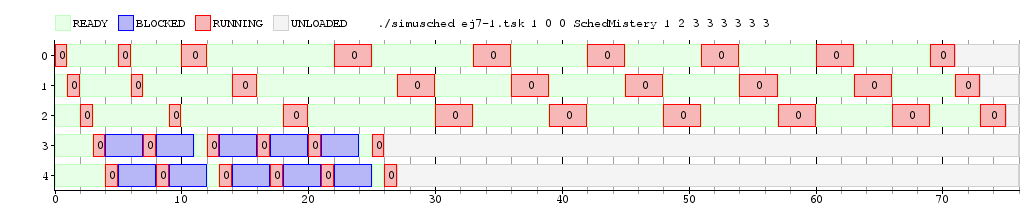
\includegraphics[width=1\textwidth]{ej7-lote1}
    \caption{Ejecución Lote 1}
    \label{Lote1}
\end{figure}

Lo que nos dice la figura \ref{Lote1} es que este scheduler hace round-robin sobre los procesos que ejecuta y además prioriza las tareas desbloqueadas por sobre el resto. También vemos que los quantum van increciendo hasta 3, correspondiendose con los parámetros pasados al scheduler `1 2 3 3 3 3 3 3`. Esto habla de la necesidad de al menos 2 colas de prioridad para manejar los niveles de prioridad para los casos de desbloqueo y la nacesidad de utilizar un algoritmo de round-robin para el intercambio de tareas.

\bigskip

\textbf{Lote 2}

TaskAlterno 3 22 1 3 3
@1
TaskAlterno 7 10 3

@20
TaskCPU 5
@22
TaskCPU 5

@30
TaskCPU 5
@32
TaskCPU 5

\begin{figure}[h]
    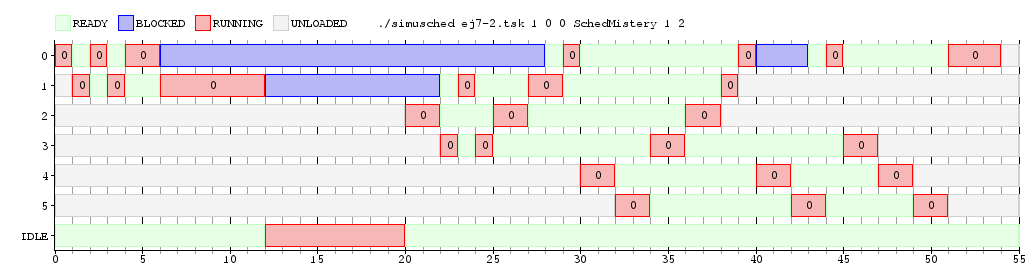
\includegraphics[width=1\textwidth]{ej7-lote2}
    \caption{Ejecución Lote 2}
    \label{Lote2}
\end{figure}

Un punto importante en la determinación del comportamiento del SchedMistery está relacionada con la inicialización de tareas. Lo que determinamos a través de la ejecución de este lote, y el posterior análisis de la figura \ref{Lote2}, es que los procesos inicializan con la mayor prioridad posible. También comprobamos que la suba de prioridad del desbloqueo se complementa con el de incialización de tareas.

\bigskip

\textbf{Lote 3}

*2 TaskCPU 10
@5
*2 TaskCPU 10
@10
*2 TaskCPU 10

\begin{figure}[h]
    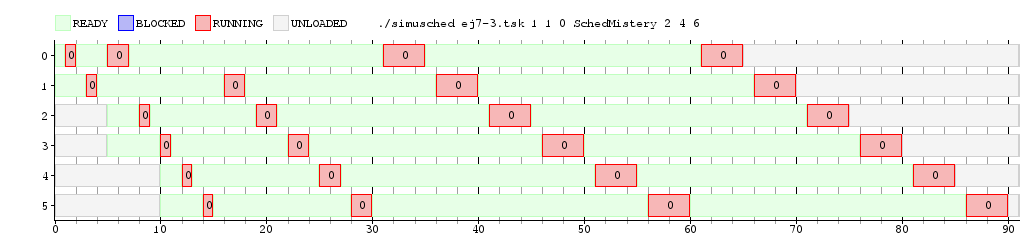
\includegraphics[width=1\textwidth]{ej7-lote3}
    \caption{Ejecución Lote 3}
    \label{Lote3}
\end{figure}

Lo que determina este lote, que se podía intuir en los lotes anteriores, es que las colas de prioridad tienen un quantum que se corresponde con los parámetros pasados al scheduler y, agregando a lo conocido por el Lote 1, por cada parámetro existe una cola de prioridad donde los procesos se van encolando. Es así que logramos comprender como funciona el Scheduler.

Creamos una batería de lotes de tests para contemplar otros casos posibles y logramos el mismo comportamiento con nuestra implementación de SchedNoMystery que el de SchedMistery. Sin embargo los 3 casos más emblemáticos son los anteriormente detallados, cumpliendo con la consigna de hablar de los 3 lotes más significativos.
